\cleardoublepage

\chapter{Shaders Gráficos}
\label{makereference3}

Como se ha visto en la sección~\ref{makereference2.3}, el pipeline de gráficos
de OpenGL tiene cuatro etapas programables:

\begin{itemize}
		\item Shader de Vértices (Vertex Shader)
		\item Shaders de Teselación
				\subitem Shader de Control de Teselación (Tessellation Control
				Shader)
				\subitem Shader de Evaluación de Teselación (Tessellation
				Evaluation Shader)
		\item Shader Geométrico (Geometry Shader)
		\item Shader de Fragmento (Fragment Shader)
\end{itemize}

Los shaders gráficos son un tipo de programa utilizado inicialmente para
producir niveles apropiados de luz, oscuridad y color en una imagen. Sin
embargo, hoy en día se utilizan con diversas finalidades diferentes como efectos
especiales, post procesado de vídeos, videojuegos, etc.

Los shaders se introdujeron en OpenGL en la versión 2.0, incluyendo el lenguaje
de programación centrado en shaders OpenGL Shading Language, también conocido
como GLSL~\cite{GLSL}--- un lenguaje tipo C creado específicamente para que los
desarrolladores tuviesen más control sobre el pipeline de renderizado.---

Durante el proceso de desarrollo de shaders no es necesario incluir todas las
etapas que se muestran en la Figura~\ref{fig2.2b}, aunque normalmente, si se
decide utilizar alguno de ellos, se requiere utilizar, al menos, un Vertex
Shader. 

Los datos se proporcionan a los shaders de dos maneras distintas desde la
aplicación principal. La primera es proporcionando los datos necesarios para el
renderizado de vértices a la primera etapa, el Vertex Shader. A partir de ese
momento Los shaders del pipeline se comunican entre ellos mediante variables
proporcionadas por GLSL o definidas por el programador en los shaders, siendo la
salida de un shader la entrada del siguiente, como se muestra en la
Figura~\ref{fig3.1}. Un breve resumen acerca del lenguaje GLSL se incluye en el
Apéndice~\ref{ApendiceA}. 

El segundo modo de especificar datos a los shaders es mediante variables
\verb|uniform|. Estas variables se definen en los shaders. Se trata de variables
de solo lectura por parte de los shaders. Al contrario que las variables
definidas como entrada y salida de un shader a otro, estas variables toman sus
valores del programa principal cada vez que se invoca el shader.  

\begin{figure}
		\centering
		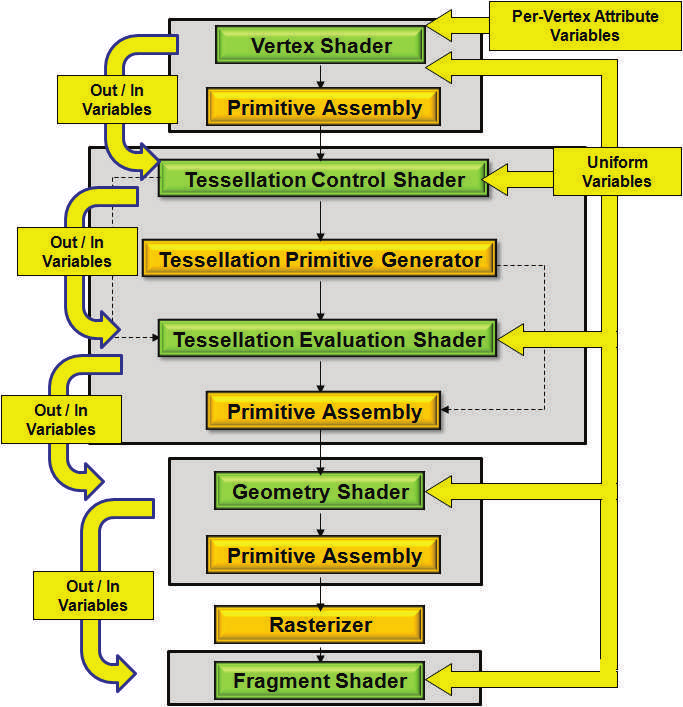
\includegraphics[height=10cm]{figures/variablespipe.png}
		\caption{Comunicación entre shaders del pipeline}
		\label{fig3.1}
\end{figure}

\section{Vertex Shader}
\label{ref:Vertex}

El Vertex Shader es la etapa de sombreado en el pipeline de renderizado que se
encarga del procesamiento de los vértices individuales~\cite{VertexShader}. El
Vertex Shader tiene como entrada unos atributos de vértice especificados desde
un \textit{Vertex Array Object (VAO)} por un comando de dibujo. Recibe un único
vértice, formado por sus atributos, del flujo de vértices y genera un único
vértice al flujo de salida. Por cada vértice de entrada ha de haber,
necesariamente, uno de salida. 

Este shader se invoca una vez por cada vértice en el flujo de entrada,
exceptuando el caso en el que OpenGL detecte que una invocación a este shader
con las exactamente las mismas entradas ya ha sido realizada, en cuyo caso se
reutilizan los resultados de la invocación previa, resultando en un ahorro
de tiempo valioso. 

Normalmente, las operaciones que se realizan en el Vertex Shader son
transformaciones para el espacio de post-proyección, iluminación por vértice o
preparación para las siguientes etapas del pipeline. 

\section{Tessellation Shaders}
\label{ref:TesShaders}

La Teselación es la etapa, opcional, del pipeline de renderizado que consiste en
subdividir un parche de algún tipo y computar los valores de los nuevos vértices
creados en el proceso. Está compuesta, a su vez, por otras tres etapas, dos de
ellas programables en forma de shader, y una intermedia fija. Cada una de estas
etapas se encarga de una parte del proceso de teselación.

En esta sección se explican los dos shaders involucrados, además de la etapa
intermedia, llamada generador de primitivas de teselación, pues resulta
importante para entender el proceso y las entradas y salidas a los shaders.

\subsection{Tessellation Control Shader}
\label{ref:TesConShader}

El Tessellation Control Shader (TCS)~\cite{TesConShader} es la primera etapa del
proceso de teselación, en el caso de ser utilizado. Se sitúa inmediatamente
posterior al Vertex Shader e inmediatamente anterior al generador de primitivas
de teselación. Controla cuánta teselación provocar en un parche determinado, así
como el tamaño del parche, permitiendo aumentar la cantidad de datos. Su función
principal es la de comunicar al generador de primitivas de teselación el nivel
de teselación deseado, así como proveerle los datos del parche al Tessellation
Evaluation Shader mediante sus variables de salida.

Como entrada, el TCS obtiene la salida del Vertex Shader organizada en un vector
de tantos vértices como tenga el parche de entrada. Cada invocación al TCS
produce un único vértice como salida al parche de salida. Por cada vértice en
el parche de entrada se realiza una invocación al TCS, resultando en tantas
invocaciones como vértices hay en dicho parche. 

En el caso de no utilizar un TCS, se pueden pasar valores por defecto a las
siguientes etapas de teselación.

\begin{figure}[t]
	\centering
	\begin{subfigure}{.45\textwidth}
		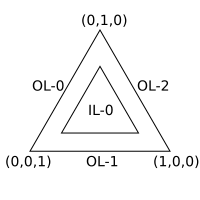
\includegraphics[width=\textwidth]{figures/TriangleLevels.png}	
		\caption{Niveles de triángulos}
		\label{fig:trilevels}
	\end{subfigure}
	\hfill
	\begin{subfigure}{.45\textwidth}
		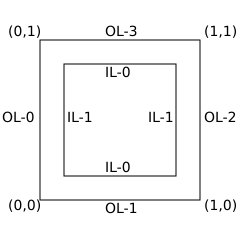
\includegraphics[width=\textwidth]{figures/QuadLevels.png}	
		\caption{Niveles de cuadriláteros}
		\label{fig:quadlevels}
	\end{subfigure}
	\par\bigskip \par\bigskip \par\bigskip
	\begin{subfigure}{.45\textwidth}
		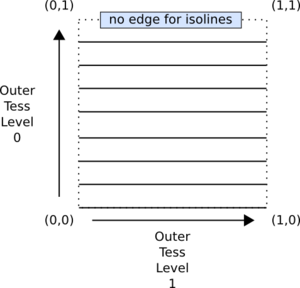
\includegraphics[width=\textwidth]{figures/300px-Tessellation_isoline.png}	
		\caption{Niveles de isolíneas}
		\label{fig:isolevels}
	\end{subfigure}
	\caption{Teselación - Funcionamiento de los niveles}
	\label{fig:tesselationlevels}	
\end{figure}

\subsection{Generador de primitivas de teselación}
\label{ref:TesPriGen}

El generador de primitivas de teselación~\cite{TesPriGen} es la etapa que se
encuentra entre los dos shaders de teselación, el TCS y el Tessellation
Evaluation Shader. Esta etapa, fija en el pipeline, es la encargada de crear
nuevas primitivas a partir del parche de entrada. La función principal de este
sistema es la de determinar cuántos vértices crear, en qué orden hacerlo y qué
clase de primitivas construir con ellos. Los datos reales de estos vértices,
como color, posición, etc., han de ser generados por el TES. Debido a esto, el
generador no tiene en cuenta el parche de salida producido por el TCS, sino que
solo opera en términos de teselar un cuadrado o triángulo abstracto, o un bloque
de isolíneas.

Esta etapa, está supeditada al Tessellation Evaluation Shader, puesto que solo
se ejecutará en el caso de que exista uno activo. La generación de primitivas en
esta etapa se ve afectada por distintos factores:

\begin{itemize}
		\item Niveles de teselación marcados por el TCS (O por defecto si no hay
				TCS)
		\item Espaciado de los vértices teselados, definido en el TES
		\item Tipo de primitiva, definido en el TES
		\item Orden de generación de primitivas, definido en el TES
\end{itemize}

La cantidad de teselación a realizar se define en niveles de teselación internos
y externos (Ver Figura~\ref{fig:tesselationlevels}). Funcionan de la siguiente
manera: un nivel de teselación 4 indica que un borde se convertirá en 4 bordes
(2 vértices se convertirán en 5). El nivel externo define el grado de teselación
para los bordes externos de la primitiva. Esto permite que dos parches distintos
se conecten apropiadamente, a pesar de tener distintos niveles de teselación
dentro del parche. El nivel interno hace referencia el número de teselaciones a
realizar dentro del parche abstracto. 

Cabe destacar que no todos los parches abstractos utilizan los mismos niveles de
teselación. Por ejemplo, los triángulos utilizan un único nivel interno y tres
niveles externos. El resto de posibles niveles son ignorados. 

El espaciado entre vértices puede realizarse de las siguientes maneras:
espaciado equidistante, espaciado fraccional par o espaciado fraccional impar.

\begin{figure}[h]
	\centering
	\begin{subfigure}{.45\textwidth}
			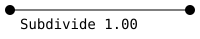
\includegraphics[width=\textwidth]{figures/equal1.png}	
	\end{subfigure}	
	\hfill
	\begin{subfigure}{.45\textwidth}
			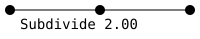
\includegraphics[width=\textwidth]{figures/equal2.png}	
	\end{subfigure}	
	\newline
	\begin{subfigure}{.45\textwidth}
			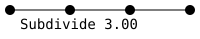
\includegraphics[width=\textwidth]{figures/equal3.png}	
	\end{subfigure}	
	\hfill
	\begin{subfigure}{.45\textwidth}
			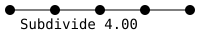
\includegraphics[width=\textwidth]{figures/equal4.png}	
	\end{subfigure}	
	\caption{Teselación - Espaciado equidistante}
	\label{fig3.2}
\end{figure}

El espaciado equidistante (ver Figura~\ref{fig3.2}) divide el borde a teselar
en segmentos de igual longitud. Solo acepta valores enteros, por lo que redondea
el nivel de teselación hasta el siguiente entero. Este hecho causa que los
segmentos aparezcan instantáneamente de un nivel a otro.

Para conseguir un comportamiento mas ``suave'' se tienen los otros dos modos de
espaciado. Estos últimos son útiles especialmente cuando el nivel de teselación
es dependiente del área vista desde la cámara. En el espaciado fraccional par el
número de segmentos en los que dividir el borde (nivel de teselación efectivo)
se redondea al siguiente entero par, mientras que en el espaciado fraccional
impar se redondea al siguiente entero impar. Para estos modos de espaciado se
necesita definir dos valores:

\begin{itemize}
		\item $n$, el nivel de teselación efectivo, redondeado según lo
				anterior.
		\item $f$, el valor computado antes del redondeo. Un valor
				potencialmente fraccionario.
\end{itemize}

\begin{figure}
	\centering
	\begin{subfigure}{.45\textwidth}
			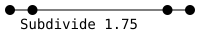
\includegraphics[width=\textwidth]{figures/even1.png}	
	\end{subfigure}
	\hfill
	\begin{subfigure}{.45\textwidth}
			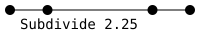
\includegraphics[width=\textwidth]{figures/even2.png}	
	\end{subfigure}
	\newline
	\begin{subfigure}{.45\textwidth}
			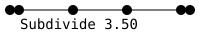
\includegraphics[width=\textwidth]{figures/even3.png}	
	\end{subfigure}
	\hfill
	\begin{subfigure}{.45\textwidth}
			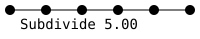
\includegraphics[width=\textwidth]{figures/even4.png}	
	\end{subfigure}
	\caption{Teselación - Espaciado fraccional par}
	\label{fig3.3}
\end{figure}

\begin{figure}
	\centering
	\begin{subfigure}{.45\textwidth}
			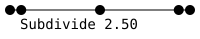
\includegraphics[width=\textwidth]{figures/odd1.png}	
	\end{subfigure}
	\hfill
	\begin{subfigure}{.45\textwidth}
			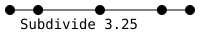
\includegraphics[width=\textwidth]{figures/odd2.png}	
	\end{subfigure}
	\newline
	\begin{subfigure}{.45\textwidth}
			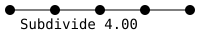
\includegraphics[width=\textwidth]{figures/odd3.png}	
	\end{subfigure}
	\hfill
	\begin{subfigure}{.45\textwidth}
			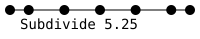
\includegraphics[width=\textwidth]{figures/odd4.png}	
	\end{subfigure}
	\caption{Teselación - Espaciado fraccional impar}
	\label{fig3.4}
\end{figure}

Según este esquema, los bordes a teselar se subdividen en dos conjuntos de
segmentos. El primero con $n-2$ segmentos de igual longitud, el otro con $2$
segmentos de igual longitud entre ellos, pero no necesariamente de igual
longitud que los del el otro conjunto. Estos dos segmentos tendrán menor
longitud que los otros en general. La longitud de estos es exactamente $n-f$.
Por tanto, cuando se cumple que $n-f=0$ se tiene que todos los segmentos tienen
igual longitud. Estos comportamientos se pueden observar en las
Figuras~\ref{fig3.3},~\ref{fig3.4}.

\subsection{Tessellation Evaluation Shader}
\label{ref:TesEvaShader}

El Tessellation Evaluation Shader (TES)~\cite{TesEvaShader} es la etapa opcional
que se encuentra entre el generador de primitivas de teselación y el geometry
shader. Su función es la de coger los resultados obtenidos en la etapa anterior
y computar las posiciones interpoladas y otros datos vértice a vértice a partir
de ellos.

El TES obtiene del generador de primitivas de teselación un parche abstracto,
así como datos de los vértices para todo el parche, junto con otros datos,
provenientes del TCS. Cada invocación a este shader produce un vértice
particular y es invocado una vez por cada vértice en el parche abstracto.

Esta es la etapa donde el programador implementa el algoritmo que se usa para
computar las nuevas posiciones, normales, coordenadas de texturas, etc. Como se
ha expuesto antes, este shader es el que determina si ocurrirá o no la etapa de
generación de primitivas de teselación, puesto que solo se ejecutará si existe
un TES activo.

El TES, en caso de ser utilizado, debe especificar el tipo de primitiva que
servirá como entrada al geometry shader. Este tipo puede ser puntos, isolíneas,
triángulos o cuadriláteros.

\begin{figure}
	\centering
	\begin{subfigure}{0.45\textwidth}
			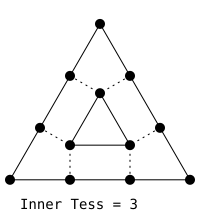
\includegraphics[height=8cm,width=\textwidth]{figures/TriInnerOnlyTriCorr.png}	
	\end{subfigure}
	\hfill
	\begin{subfigure}{0.45\textwidth}
			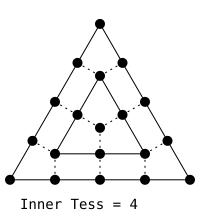
\includegraphics[height=8cm,width=\textwidth]{figures/TriInnerOnlyPointCorr.png}	
	\end{subfigure}
	\newline
	\begin{subfigure}{0.45\textwidth}
			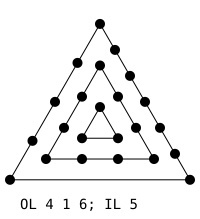
\includegraphics[height=8cm,width=\textwidth]{figures/TriOuterAndNotris.png}	
	\end{subfigure}
	\hfill
	\begin{subfigure}{0.45\textwidth}
			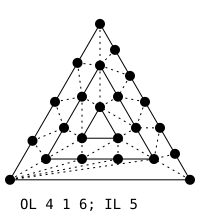
\includegraphics[height=8cm,width=\textwidth]{figures/TriFull.png}	
	\end{subfigure}
	\caption{Teselación - Triángulos}
	\label{fig:triangletessellation}
\end{figure}

\begin{figure}
	\centering
	\begin{subfigure}{0.40\textwidth}
			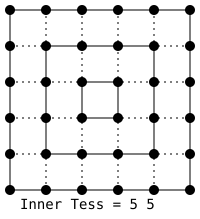
\includegraphics[height=7cm,width=\textwidth]{figures/QuadInnerOnlyQuadCorr.png}	
	\end{subfigure}
	\hfill
	\begin{subfigure}{0.40\textwidth}
			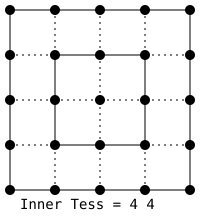
\includegraphics[height=7cm,width=\textwidth]{figures/QuadInnerOnlyPointCorr.png}	
	\end{subfigure}
	\newline
	\begin{subfigure}{0.40\textwidth}
			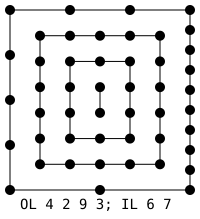
\includegraphics[height=7cm,width=\textwidth]{figures/QuadOuterAndNotris.png}	
	\end{subfigure}
	\hfill
	\begin{subfigure}{0.40\textwidth}
			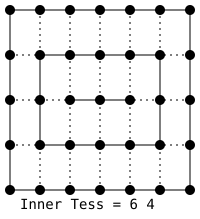
\includegraphics[height=7cm,width=\textwidth]{figures/QuadInnerOnlyLineCorr.png}	
	\end{subfigure}
	\newline
	\begin{subfigure}{0.40\textwidth}
			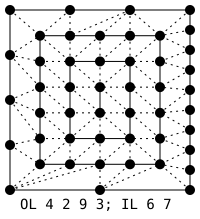
\includegraphics[height=7cm,width=\textwidth]{figures/QuadFull.png}	
	\end{subfigure}
	\caption{Teselación - Cuadriláteros}
	\label{fig:quadtessellation}
\end{figure}

\section{Geometry Shader}
\label{ref:GeoShader}

El Geometry Shader~\cite{GeoShader} es un programa escrito en GLSL que
corresponde a la etapa del pipeline programable que se encuentra entre el TES o
el Vertex Shader (dependiendo de si existe o no teselación) y la etapa fija de
post-procesado de vértices. Este shader es opcional y no es necesaria su
utilización.

Las invocaciones a este shader toman como entrada una única primitiva geométrica
y puede dar como salida cero o más primitivas, aunque existe un límite de
primitivas que se pueden generar en cada invocación, dependiendo de la
implementación. Los shaders geométricos están diseñados para aceptar como
entrada una primitiva específica y dar como salida otra. 

Sus usos varían bastante, pudiéndose utilizar como una manera de amplificar la
geometría, sirviendo como una especie de teselación, así como para realizar un
renderizado por capas o incluso para la realización de tareas de cómputo en la
GPU. 

Entre las primitivas de entrada aceptadas por el geometry shader se encuentran
las siguientes:

\begin{table}[h]
		%\centering
		\begin{tabular}{|m{4cm}|m{7cm}|m{2.2cm}|m{1.5cm}|}

			\hline
			Entrada & Primitiva & Parámetro TES & Vértices\\
			\hline

			\verb|points| & \verb|GL_POINTS| & \verb|point_mode| & 1 \\
			\hline

			\verb|lines| & \verb|GL_LINES, GL_LINE_STRIP,| \verb|GL_LINE_LIST| &
			\verb|isolines| & 2\\

			\hline

			\verb|lines_adjacency| & \verb|GL_LINES_ADJACENCY,|
			\verb|GL_LINE_STRIP_ADJACENCY| & \verb|N/A| & 4\\

			\hline

			\verb|triangles| & \verb|GL_TRIANGLES, GL_TRIANGLE_STRIP,|
			\verb|GL_TRIANGLE_FAN| & \verb|triangles,| \verb|quads| & 3 \\

			\hline

			\verb|triangles_adjacency| & \verb|GL_TRIANGLES_ADJACENCY,|
			\verb|GL_TRIANGLE_STRIP_ADJACENCY| & \verb|N/A| & 6 \\

			\hline
		\end{tabular}
		\caption{Primitivas de entrada al Geometry Shader}
		\label{tabla3.1}
\end{table}

Las primitivas de salida pueden ser únicamente alguna de las siguientes:

\begin{itemize}
		\item \verb|points|	
		\item \verb|line_strip|
		\item \verb|triangle_strip|
\end{itemize}

Los shaders geométricos pueden generar tantos vértices como permita el límite de
implementación. Para ello, el programador genera los valores que necesite para
el nuevo vértice y, una vez estos valores sean correctos, una llamada a la
función \verb|EmitVertex()| produce el vértice deseado. Una vez llamada esta
función, los valores escritos para el vértice son reseteados, teniendo que
volver a escribirlos para generar otro vértice. 

De igual modo, para generar una primitiva, debemos especificar del modo anterior
todos los vértices que forman esa primitiva y posteriormente llamar a la función
\verb|EndPrimitive()|. De esta forma, si se desea generar más de una primitiva,
se deben especificar los vértices que forman la primera, llamar a
\verb|EndPrimitive()|, generar los vértices que forman la segunda y llamar de
nuevo a \verb|EndPrimitive()| para generar la segunda primitiva.

\section{Fragment Shader}
\label{ref:FragShader}

El Fragment Shader~\cite{FragShader} es la etapa posterior a la rasterización.
Por cada uno de los píxeles cubiertos por una primitiva, se genera un fragmento.
Cada uno de estos fragmentos tiene una posición en la espacio de ventana, así
como otros valores procedentes de la etapa de procesamiento de vértices.

La salida del fragment shader consta de un valor de profundidad, un posible
valor de plantilla (que no es modificado por el shader) y cero o más valores de
color para ser potencialmente escritos en los buffers del frame buffer actual.
Estos shaders toman como entrada un único fragmento, producido por el
rasterizador, y dan como salida otro único fragmento. 

Técnicamente, la utilización de estos shaders es también opcional, puesto que de
no utilizarlo, los valores de color del fragmento de entrada quedarán
indefinidos, pero los valores de profundidad y plantilla en la salida serán los
mismos que los de entrada. Esto puede ser interesante en el caso de solo estar
interesados en los valores de profundidad computados por el sistema en lugar de
otro valor calculado por el programador. 

Este shader también tiene operaciones especiales no presentes en los otros tipos
de shader, como puede ser la instrucción \verb|discard|, cuyo objetivo es
descartar los valores de salida generados durante la ejecución del shader para
un fragmento en concreto, haciendo que este fragmento no pase a las siguientes
etapas del pipeline. Esto puede ser útil para descartar fragmentos cuyos valores
generados en la ejecución se queden fuera de unos límites impuestos por el
programador.
